\chapter{Visual design}\label{ch:visualDesign}
\section{Concept art}
Concept art was created for several iterations of the player-controlled pirate characters, some of which is seen in Figure \ref{fig:pirate_concepts}. They were drawn with a simple, cartoonish look in mind, so that the characters easily catch the players' eyes. 

\begin{figure}[h!]
    \centering
    \begin{subfigure}[b]{0.2\textwidth}
		\centering        
        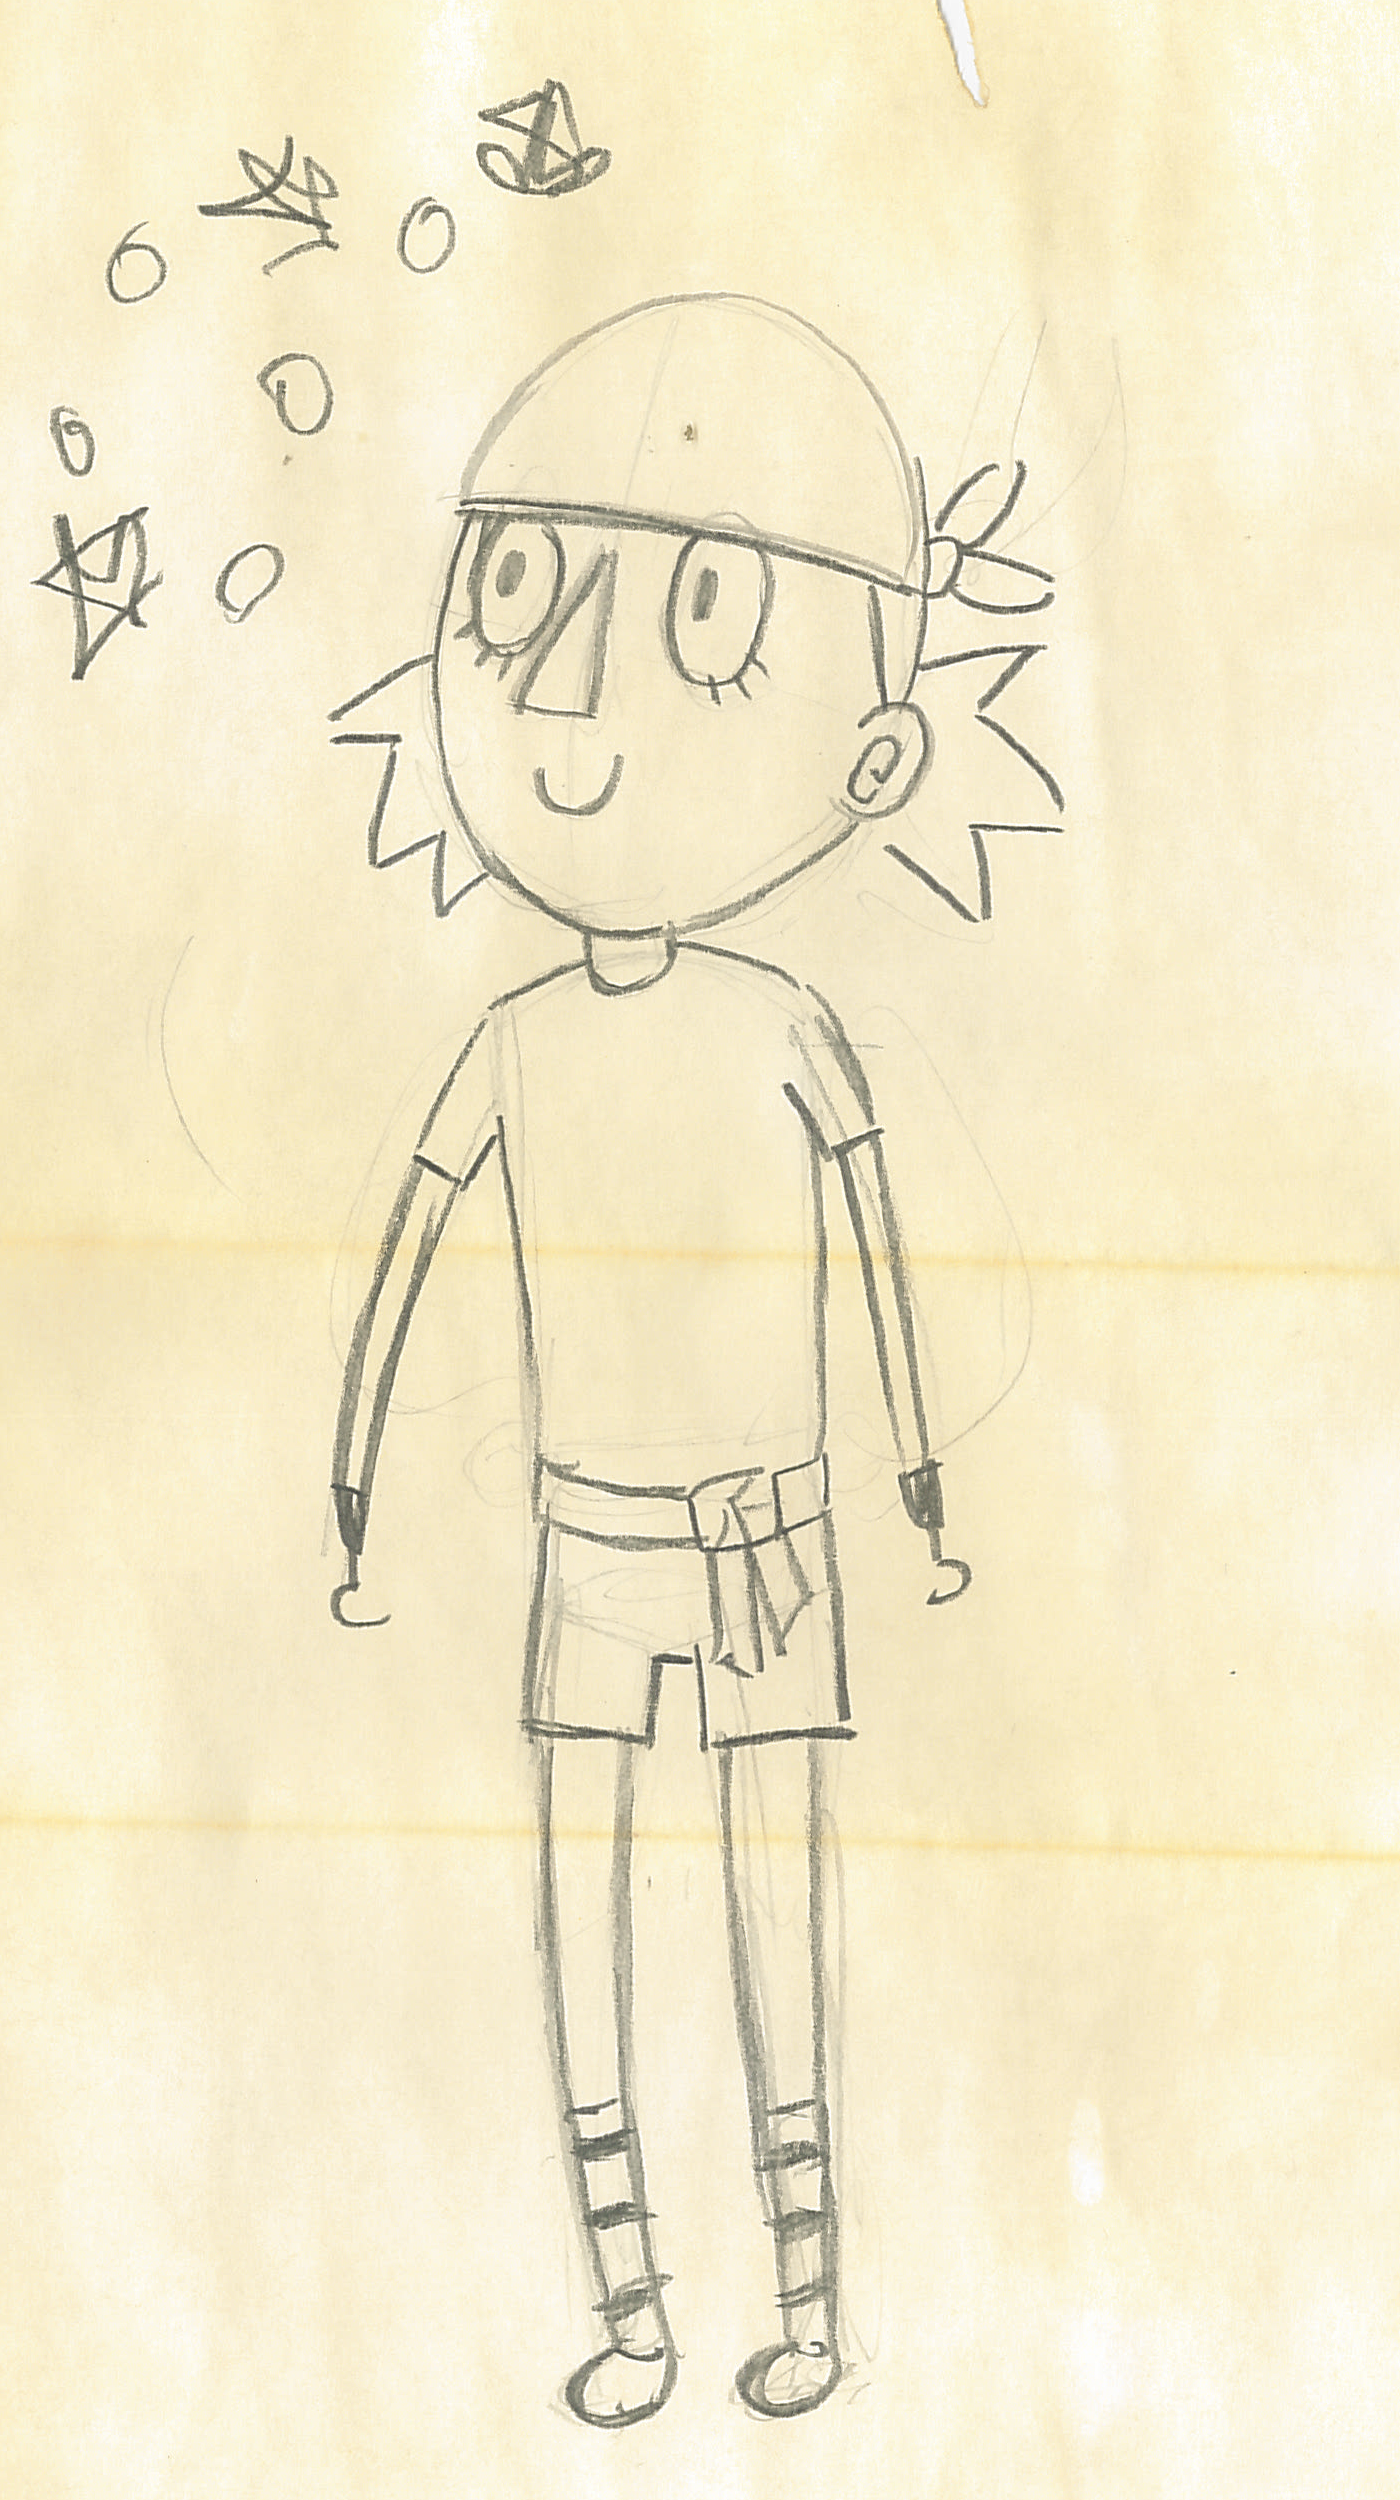
\includegraphics[width=\textwidth]{figures/pirate_concept_0.png}\caption{ \label{fig:pirate_concept_0}}
    \end{subfigure}
    \begin{subfigure}[b]{0.2\textwidth}
    	\centering
        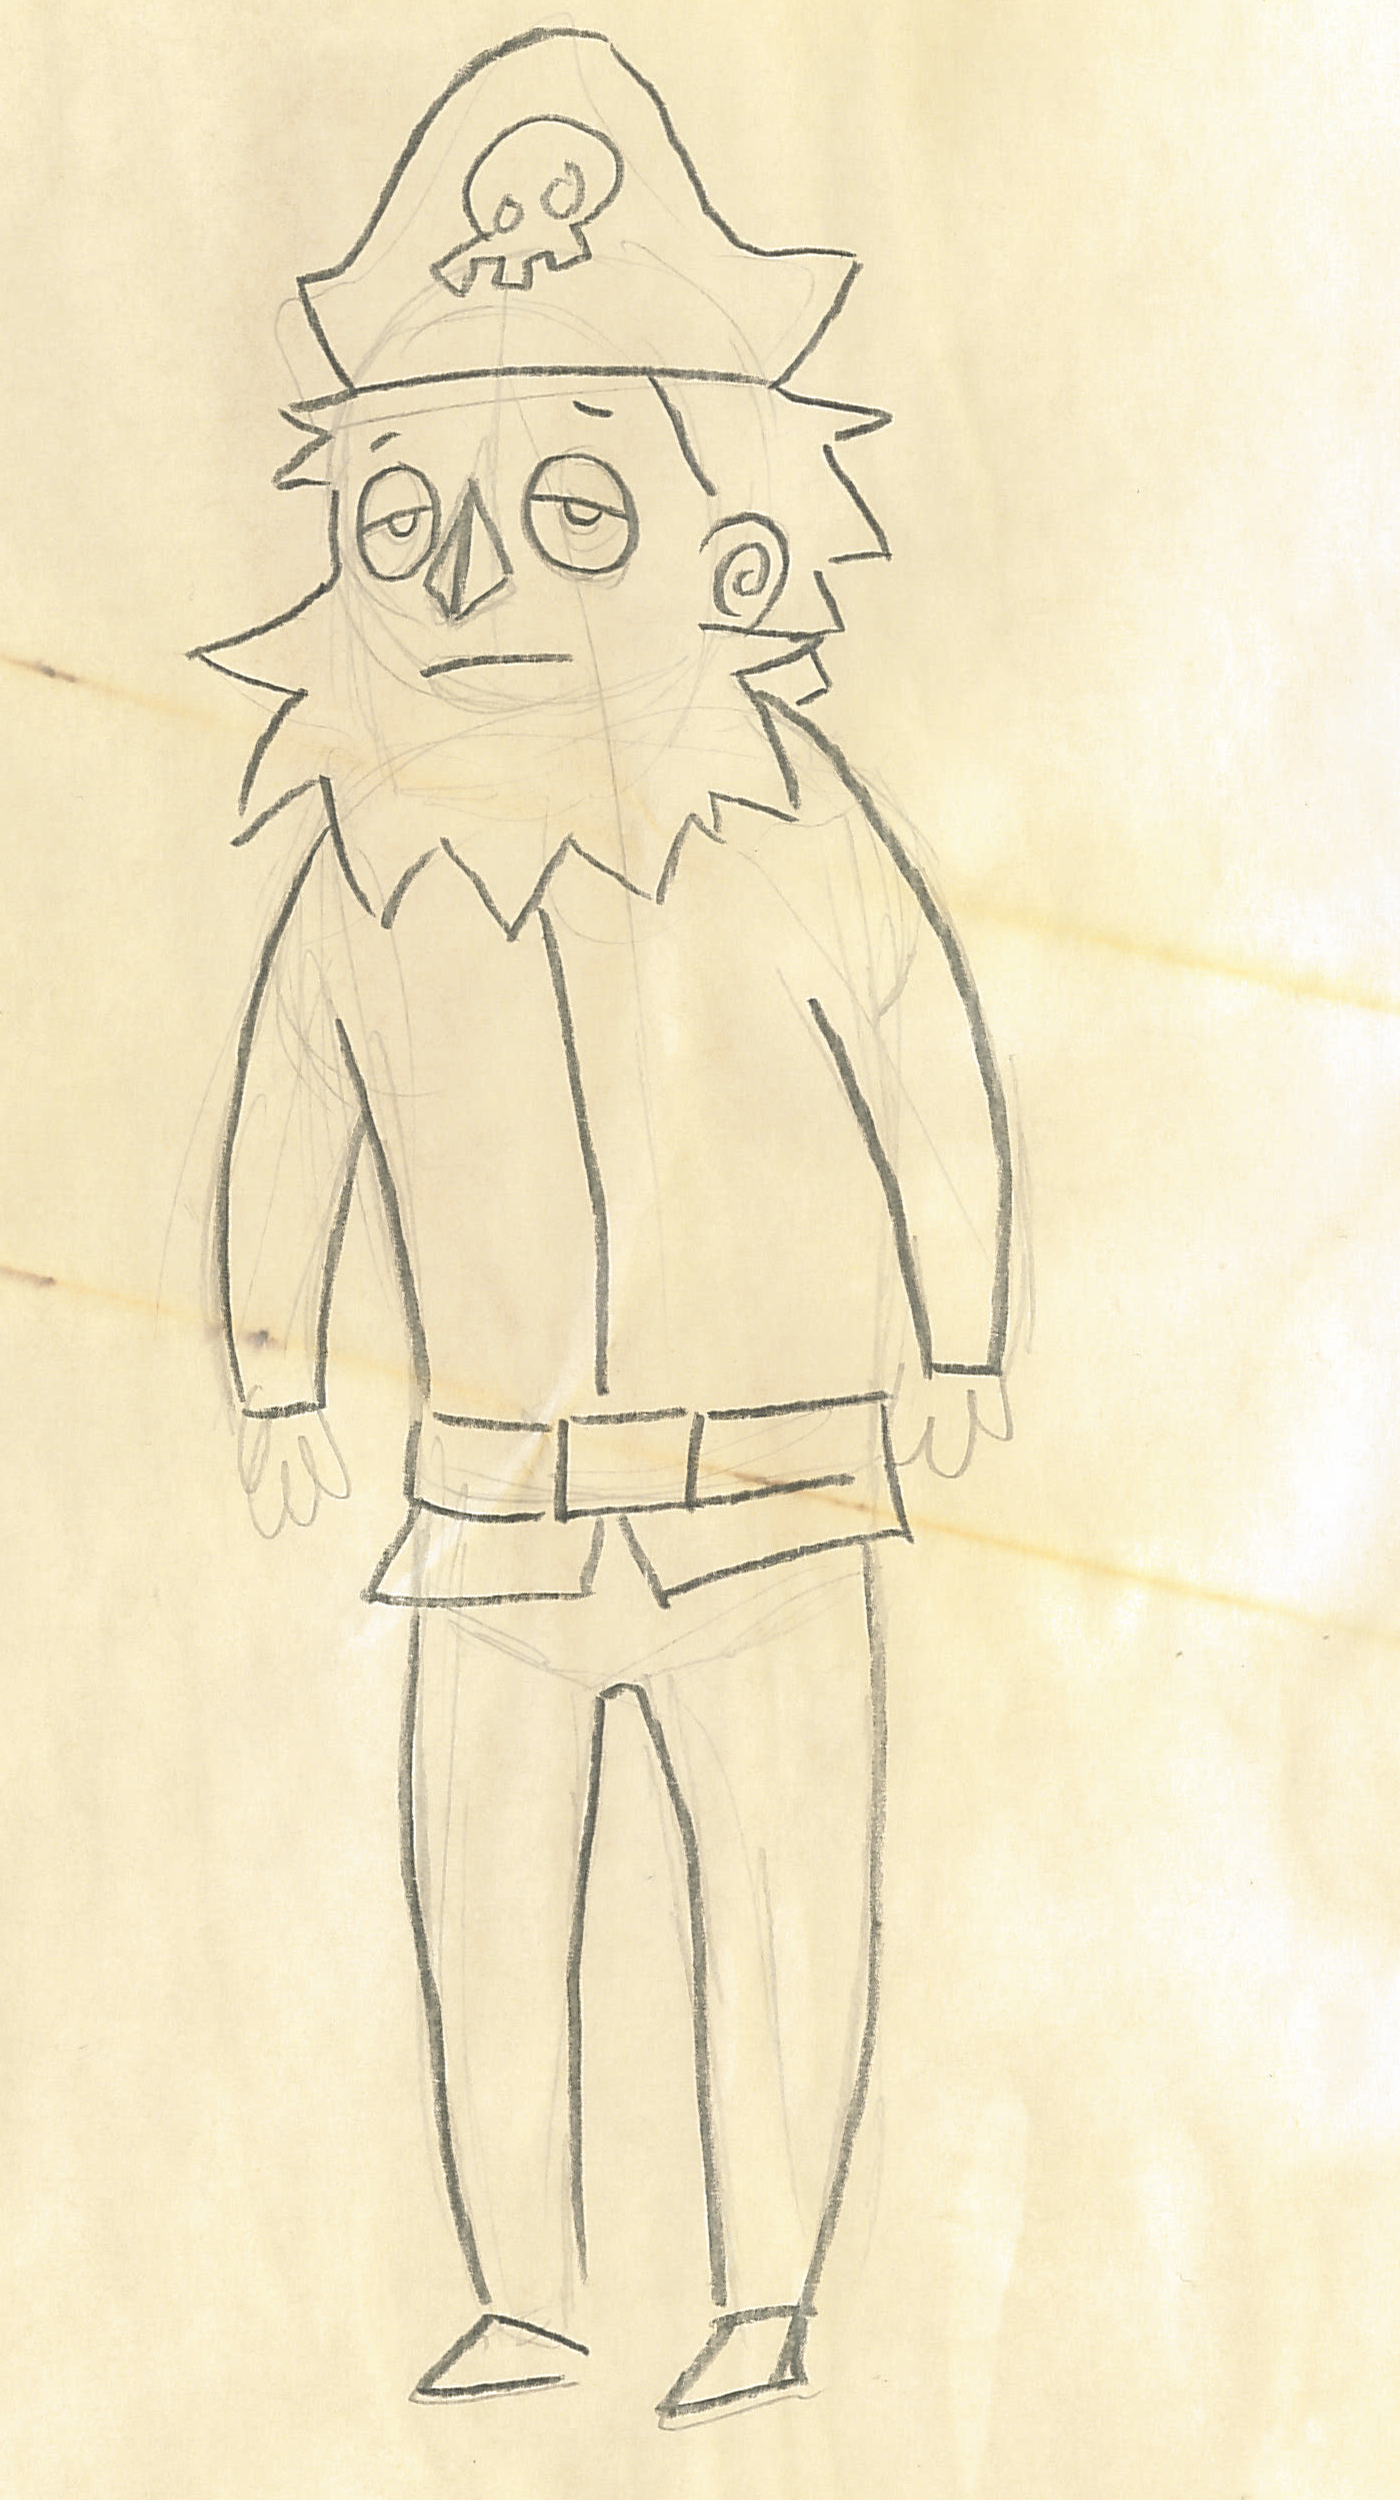
\includegraphics[width=\textwidth]{figures/pirate_concept_1.png}\caption{ \label{fig:pirate_concept_1}}
    \end{subfigure}
    \begin{subfigure}[b]{0.2\textwidth}
    	\centering
        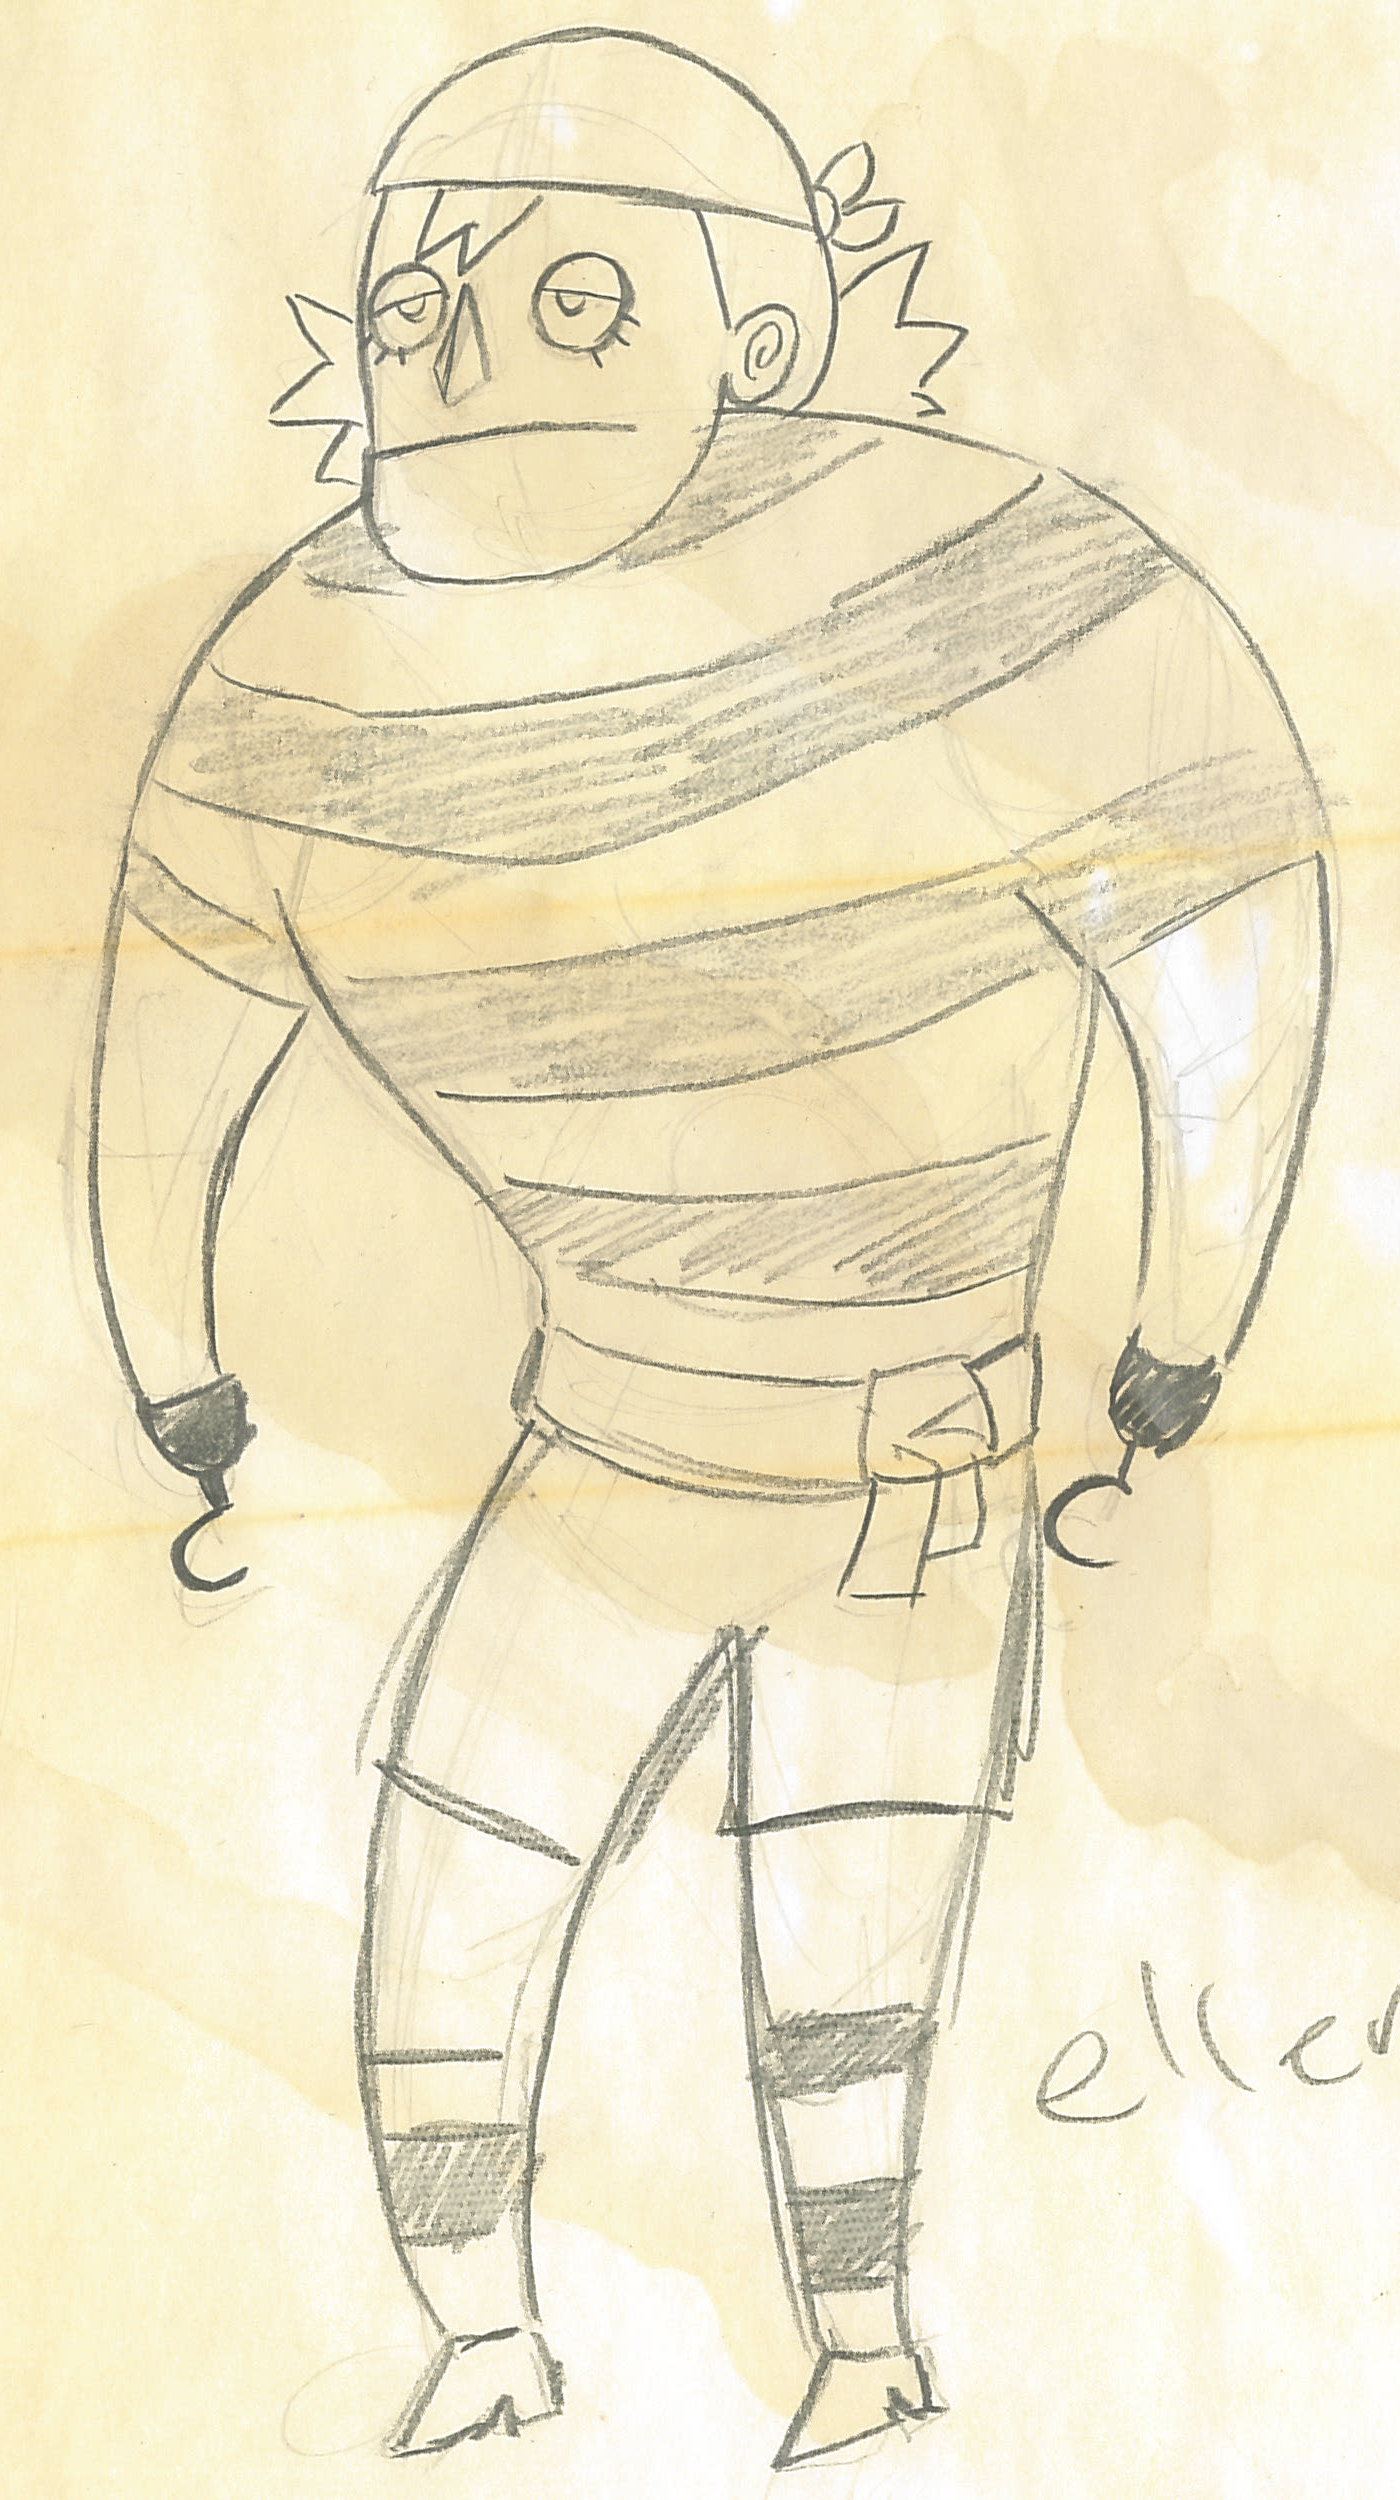
\includegraphics[width=\textwidth]{figures/pirate_concept_2.png}\caption{ \label{fig:pirate_concept_2}}
    \end{subfigure}
    \begin{subfigure}[b]{0.2\textwidth}
    	\centering
        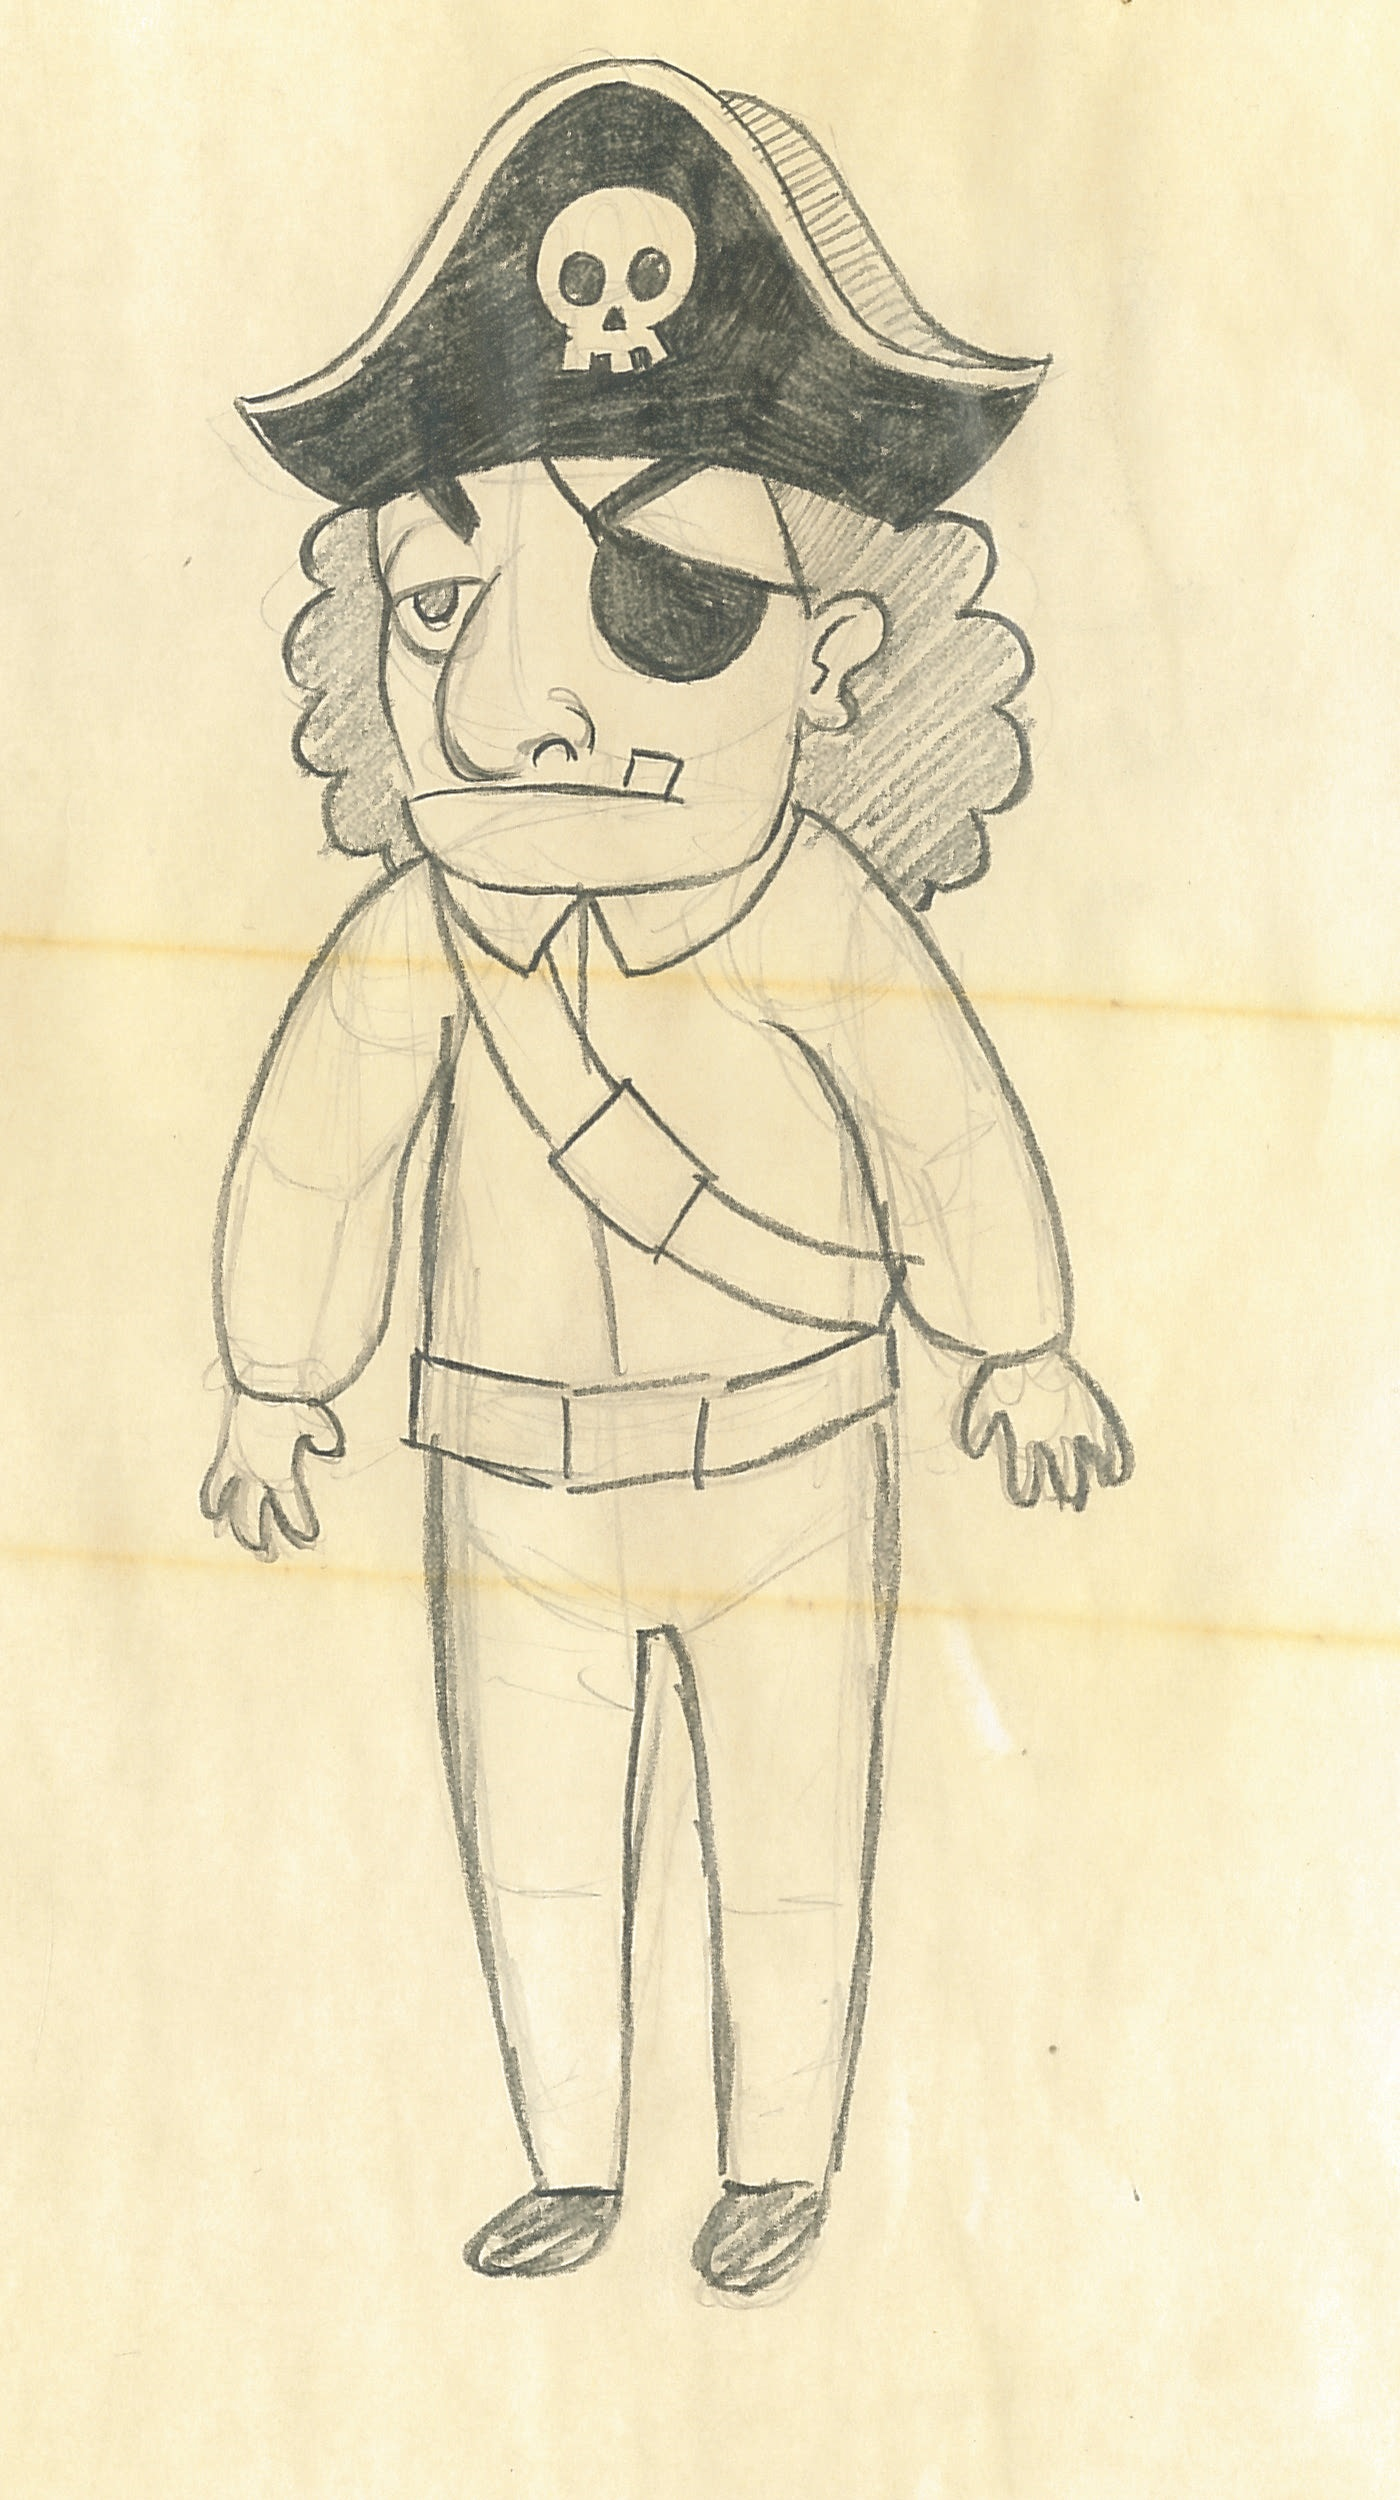
\includegraphics[width=\textwidth]{figures/pirate_concept_3.png}\caption{ \label{fig:pirate_concept_3}}
    \end{subfigure}
    \caption{Concept art of the pirate characters}\label{fig:pirate_concepts}
\end{figure}

In the end, the concept pictured in Figure \ref{fig:pirate_concept_2} was decided upon, in part due to its large torso; if the shirt and bandana are a certain colour, that colour will take up a relatively large percentage of the character's surface, allowing for it to be easily seen by the players, even when several characters are on the screen. 

\section{3D graphics}

\subsection{Modeling}
The models for this game are built and animated using Autodesk Maya, and consist of transformed primitives, such as spheres and cylinders. For example, the head of the player-controlled pirate character is a transformed sphere, and the torso as well as the limbs consist of cylinders. The trunks of the palm trees are created from cylinders, and their leaves from planes. All four pirate characters have identical meshes, seen in Figure \ref{fig:pirate_mesh}.

\begin{figure}[h!]
	\centering
	\includegraphics[width=0.9\textwidth]{figures/pirate_mesh.png}
	\caption{Pirate mesh: front, side and back view \label{fig:pirate_mesh}}
\end{figure}

The components of the pirate mesh were transformed based on two reference images of the character design, assigned to two image planes, one showing a frontal view of the character, and one showing a side view. These planes can be seen in Figure \ref{fig:pirate_planes}. However, small changes were made during modeling, such as the short pigtails, which were changed into longer braids in the final version.

\begin{figure}[h!]
	\centering
	\includegraphics[width=0.7\textwidth]{figures/pirate_planes.png}
	\caption{Pirate mesh: front, side and back view \label{fig:pirate_planes}}
\end{figure}

The interactive objects were not created using this technique, but rather modelled "free-hand". Like the character, the design of these objects aim for simplicity rather than realism.

\subsection{Textures}
Each pirate is assigned a \textit{lambert} material with a simple texture applied to it. The textures are very similar (simple face, light skin, neutrally coloured shorts), but they differ in the colour of each pirate's bandana and shirt colour. The colours of the four characters are red, green, yellow, and blue, as pictured in figure \ref{fig:pirate_rainbow}. The green colour specifically is chosen so that it is not too similar to the yellow colour --- the two were reviewed by a colour deficient person, who often has trouble discerning between light green and yellow colours. This person was able to easily discern between the yellow and green pirates.

\begin{figure}[h!]
	\centering
	\includegraphics[width=\textwidth]{figures/pirate_rainbow.png}
	\caption{All four player colours \label{fig:pirate_rainbow}}
\end{figure}

The texture was applied to the pirates using UV mapping; the geometry is flattened onto a two-dimensional coordinate system. Based on this flattened-out UV-map, an image containing all the necessary colours was created. An example of such a UV map (specifically for the red pirate) is seen in Figure \ref{fig:uv_map}.

\begin{figure}[h!]
	\centering
	\includegraphics[width=\textwidth]{figures/uv_map.png}
	\caption{The UV map for a pirate \label{fig:uv_map}}
\end{figure}

The interactive objects have likewise been textured. These objects can be seen in Figure \ref{fig:objects}.

\begin{figure}[h!]
    \centering
    \begin{subfigure}[b]{0.3\textwidth}
    	\centering
        \includegraphics[scale=0.2]{figures/fern.png}\caption{A fern\label{fig:fern}}
    \end{subfigure}
    \begin{subfigure}[b]{0.3\textwidth}
    	\centering
        \includegraphics[scale=0.2]{figures/skull.png}\caption{A skull\label{fig:skull}}
    \end{subfigure}
    \begin{subfigure}[b]{0.3\textwidth}
    	\centering
        \includegraphics[scale=0.2]{figures/PalmTree.png}\caption{A palm tree\label{fig:palmtree}}
    \end{subfigure}
\caption{The interactive objects}\label{fig:objects}
\end{figure}

\pagebreak
\section{Rigging and animation}
In order to animate the models, they have all been rigged. A skeleton is created and assigned to a model, with joints at the places where the model in question should be able to bend. For example, the pirate model seen in Figure \ref{fig:rigged_pirate} has a skeleton assigned to it, with joints at its shoulders, wrists, knees, et cetera.

Once the skeleton is built, each joint's \textit{weight} is painted onto the model. The weight of a joint controls which parts of the body move as the joint is rotated, and how much. Figure \ref{fig:elbow_pirate} shows weights painted in the pirate's left elbow. Furthermore, limits are set for each joint so that they don't bend too far, or bend in the wrong direction. For example, the pirate's knees can only bend on the y-axis, and only towards the rear.

\begin{figure}[h!]
	\centering
	\begin{subfigure}[b]{0.45\textwidth}
		\centering
		\includegraphics[scale=0.6]{figures/rigged_pirate.png}
		\caption{The rigged skeleton}
		\label{fig:rigged_pirate}
	\end{subfigure}
	\begin{subfigure}[b]{0.45\textwidth}
		\centering
		\includegraphics[scale=0.6]{figures/elbow_pirate.png}
		\caption{The pirate's elbow, with weights}
		\label{fig:elbow_pirate}
	\end{subfigure}
	\caption{A rigged version of the pirate model}
	\label{fig:riggin}
\end{figure}

With the skeleton properly set up, the model can be posed in different positions, allowing for animation using key frames. Key frames mark the start and end points of a smooth transition between two poses. For this projects, the models are posed in Autodesk Maya, which automatically generates a smooth transition once the key frames have been set. When setting the key frames, the model is posed using the rigged joints. The pirate model has three animations with 4-6 key frames, all of which can be seen in Figure \ref{fig:key_frames}. Likewise, the interactive objects each have an animation which will play when they are searched.

\begin{figure}[h!]
	\centering
	\begin{subfigure}[b]{\textwidth}
		\centering
		\includegraphics[scale=0.2]{figures/walk_cycle.png}
		\caption{Walk cycle}
		\label{fig:walk_cycle}
	\end{subfigure}
	
	\begin{subfigure}[b]{\textwidth}
		\centering
		\includegraphics[scale=0.2]{figures/attack_anim.png}
		\caption{Attack animation}
		\label{fig:attack_anim}
	\end{subfigure}
	
	\begin{subfigure}[b]{\textwidth}
		\centering
		\includegraphics[scale=0.2]{figures/search_anim.png}
		\caption{Search animation}
		\label{fig:search_anim}
	\end{subfigure}
	\caption{Key frames for the animations of the pirate}
	\label{fig:key_frames}
\end{figure}

\section{Interface elements}
For the purposes of testing different types of feedback on two screens, several images for visual feedback have been created. The images signalling that it is now a certain player's turn consist mainly of that player's colour, as seen in Figure \ref{fig:yellow_turn}, in which the yellow player's signal is shown. The intent is that the player's attention is quickly drawn to the image, and that it is quickly communicated that it is a given player's turn.

\begin{figure}[h!]
	\centering
	\includegraphics[width=0.7\textwidth]{figures/yellowturn.png}
	\caption{Visual feedback for yellow player's turn}
	\label{fig:yellow_turn}
\end{figure}

When a fight is about to commence, another image, seen in Figure \ref{fig:get_ready}, shows up. It is black, with highly contrasting colours, in order to quickly catch the players' eyes without being biased in any player's direction.

\begin{figure}[h!]
	\centering
	\includegraphics[width=0.7\textwidth]{figures/getready.png}
	\caption{Visual feedback warning players that a fight will commence}
	\label{fig:get_ready}
\end{figure}

The actual fighting screen which appears during a fight sequence between two players is unsaturated. Ideally, by this point, the player's attention is already aimed at the phone screen, either nudged by the tactile feedback or the "Get ready to FIGHT!" image, depending on the test. The fighting screen can be seen in Figure \ref{fig:fight}.\todo{add some stuff about the buttons as well}

\begin{figure}[h!]
	\centering
	\includegraphics[width=0.7\textwidth]{figures/fight.png}
	\caption{The fight screen}
	\label{fig:fight}
\end{figure}\todo{replace the FIGHT! image later later}

\todo{Add some stuff about the general interface}

\section{Phone interface}
The smart phone has three primary screens besides the fight screen: the planning screen, the waiting screen and the map screen. Only two out of the three were complete at the end of this project, the planning and the waiting screen. 

\begin{figure}[h!]
	\centering
	\includegraphics[width=0.7\textwidth]{figures/planningScreen.png}
	\caption{The planning screen}
	\label{fig:plan}
\end{figure}


\begin{figure}[h!]
	\centering
	\includegraphics[width=0.7\textwidth]{figures/waitingScreen.png}
	\caption{The waiting screen}
	\label{fig:wait}
\end{figure}